\sect{Komplexitätstheorie}

Theorie der quantitativen Gesetze und Grenzen der algorithmischen Informationsverarbeitung.
\begin{itemize}
    \item Zeitkomplexität: Laufzeit des besten Programms, welches das Problem löst
    \item Platzkomplexität: Speicherplatzbedarf des besten Programms
    \item Beschreibungskomplexität: Länge des kürzesten Programms
\end{itemize}

Sei $M$ eine TM, die immer hält, und sei $\omega \in \Sigma^*$.
Der Zeitbedarf von $M$ auf der Eingabe $\omega$ ist:\\
$\texttt{Time}_M(\omega) =$ Anzahl von Konfigurationsübergängen der Berechnung von $M$ auf $\omega$.

Der \textbf{Zeitbedarf} von $M$ auf Eingaben der Länge $n \in \N$ im schlechtesten Fall ist definiert als:\\
$\texttt{Time}_M(n) = \max\{\texttt{Time}_M(\omega) \mid |\omega| = n\}$

\ssect{Asymptotische Komplexität}

Seien $f,g: \N \rightarrow \N$ zwei Funktionen.
Dann gilt:
\begin{itemize}
    \item $f \in \bigO(g)$: Es existieren $n_0 \in \N$ und $c \in \N$, sodass $\forall n \geq n_0$ gilt:\\
    $f(n) \leq c \cdot g(n)$\\
    ($f$ wächst asymptotisch nicht schneller als $g$)
    \item $f \in \Omega(g)$: Es existieren $n_0 \in \N$ und $d \in \N$, sodass $\forall n \geq n_0$ gilt:\\
    $f(n) \geq \frac{1}{d} \cdot g(n)$
    ($f$ wächst asymptotisch mindestens so schnell wie $g$)
    \item $f \in \Theta(g)$: Es gilt $f(n) \in \bigO(g(n))$ und $f(n) \in \Gamma(g(n))$\\
    ($f$ und $g$ sind asymptotisch gleich)
\end{itemize}

\textbf{Beispiel:}

$\displaystyle \bigO(1) \subset \bigO(n \cdot \log(n)) \subset \bigO(1000 + n^2) \\
\subset \bigO(n^2 \cdot \log(n) + 99) \subset \bigO\left(n^{\frac{5}{2}}\right) \\
\subset \bigO(3^n + n^2) \subset \bigO(5^{n + 3}) \subset \bigO(3^{n!})$

\columnbreak

\textbf{Rechenregeln:}
\begin{itemize}
    \item Konstante Vorfaktoren kann man ignorieren: $c \cdot f(n) \in \bigO(f(n))$
    \item Für eine Konstante $c$ gilt: $c \in \bigO(1)$
    \item Bei Polynomen ist nur die höchste Potenz entscheidend:\\
    $a_k n^k + a_{k-1} n^{k-1} + \dots + a_1 n + a_0 \in \bigO(n^k)$
    \item Die $\bigO$-Notation ist transitiv:\\
    Aus $f(n) \in \bigO(g(n))$ und $g(n) \in \bigO(h(n))$ folgt $f(n) \in \bigO(h(n))$
\end{itemize}

\textbf{Bemerkung:} $\bigO(g(n))$ ist die \emph{Menge} aller Funktionen $f(n)$, für die es zwei Konstanten $n_0$ und $c$ gibt, sodass $\forall n \geq n_0$ gilt: $f(n) \leq c \cdot g(n)$

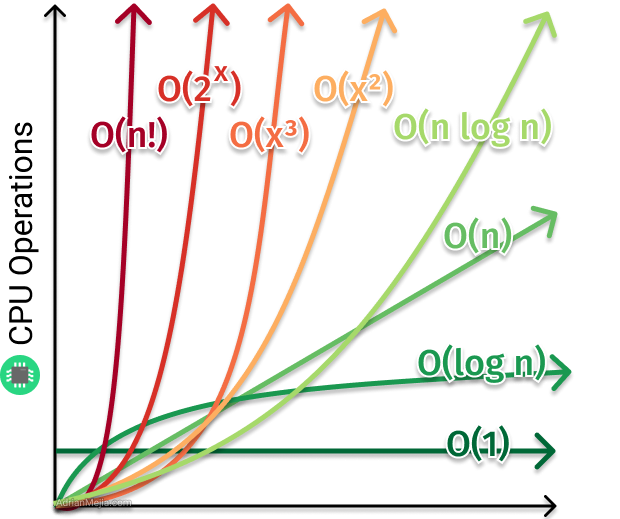
\includegraphics[scale=0.28]{time-complexity}

\ssect{Klassifizierung von Problemen}

Ein Problem $U$ heisst \textbf{in Polynomzeit lösbar}, wenn es eine obere Schranke $\bigO(n^c)$ gibt für eine Konstante $c \geq 1$.

Die \textbf{Klasse aller in Polynomzeit entscheidbaren Sprachen} wird \textbf{P} genannt.

Die \textbf{Klasse aller von einer NTM in Polynomzeit entscheidbaren Sprachen} nennen wir \textbf{NP}. \textbf{NP} heisst ``\emph{nichtdeterministisch polynomiell}''.

\textbf{Satz:} NP ist die Menge aller Sprachen, für die ein Polynomzeit-Verifizierer existiert.
\begin{itemize}[label={}]
    \item \textbf{P} = Lsg \emph{finden} in Polynomzeit
    \item \textbf{NP} = Lsg \emph{verifizieren} in Polynomzeit
\end{itemize}

\sssect{NP-Schwer \& NP-vollständig}

Eine Sprache $L$ heisst \textbf{NP-Schwer}, falls es für alle Sprachen $L' \in NP$ gilt: $L' \preceq_p L$

D.h.\ $L$ ist bezüglich der Lösbarkeit in polynomieller Zeit mindestens so schwer wie jedes einzelne Problem in NP

Eine Sprache $L$ heisst \textbf{NP-vollständig}, falls $L \in NP$ und $L$ NP-schwer ist.

Die Menge der NP-vollständigen Sprachen betrachten wir als die gesuchte Teilklasse von schwersten Entscheidungsproblemen in NP.\

\textbf{Nachweis der NP-Schwere}
\begin{enumerate}
    \item Finde ein erstes NP-schweres Problem
    \item Finde eine Polynomzeitreduktion von einem bekannten NP-schweren Problem auf das neue Problem, dessen NP-Schwere gezeigt werden soll.
\end{enumerate}

\textbf{Nachweis der NP-Vollständigkeit}
\begin{enumerate}
    \item Zeige, dass das Problem NP-Schwer ist.
    \item Zeige, dass das Problem in NP liegt.
\end{enumerate}

\textbf{Satz:}
Wenn $P_1$ NP-schwer und $P_2$ in NP enthalten ist und eine polynomielle Reduktion $P_1 \preceq_p P_2$ existiert, dann ist $P_2$ NP-vollständig.

\vspace{-\baselineskip}
\hrulefill

